\chapter{Derivados de los ácidos carboxílicos}\label{ch:b2:acyl-substitution}

Hiérvase aceite de oliva con hidróxido de sodio y se obtienen jabón y glicerol: la
reacción orgánica más antigua realizada a propósito. El aceite es un éster del glicerol y de
ácidos de cadena larga, y el hidróxido corta cada éster por un enlace, siempre el
mismo, entre el carbono carbonílico y el oxígeno del alcohol. Los ésteres,
los ácidos, las amidas, los anhídridos y los \omterm{def:b2:acyl-substitution:derivative}{cloruros de acilo} reaccionan todos de este modo: un
nucleófilo se adiciona al carbono carbonílico, y un grupo sale. Ordenar estos
compuestos según lo bien que sale su grupo indica cuáles pueden convertirse en cuáles,
y en qué sentido el químico debe ir cuesta arriba.

\begin{recall}
El volumen del primer año: activación electrófila de un grupo carbonilo, mecanismos de formación de hemiacetales y
acetales, adiciones de organomagnesianos, dadores de hidruro y su alcance, grupos salientes,
$\mathrm pK_a$, $Q$ y $K$. \Cref{ch:b2:amines}: \omterm{def:b2:amines:nucleophilic-addition}{adición nucleófila}, aminas.
\Cref{ch:b2:equilibrium-shifts}: desplazar un equilibrio. El volumen escolar: ésteres, ácidos carboxílicos
y amidas.
\end{recall}

\begin{omfigure}
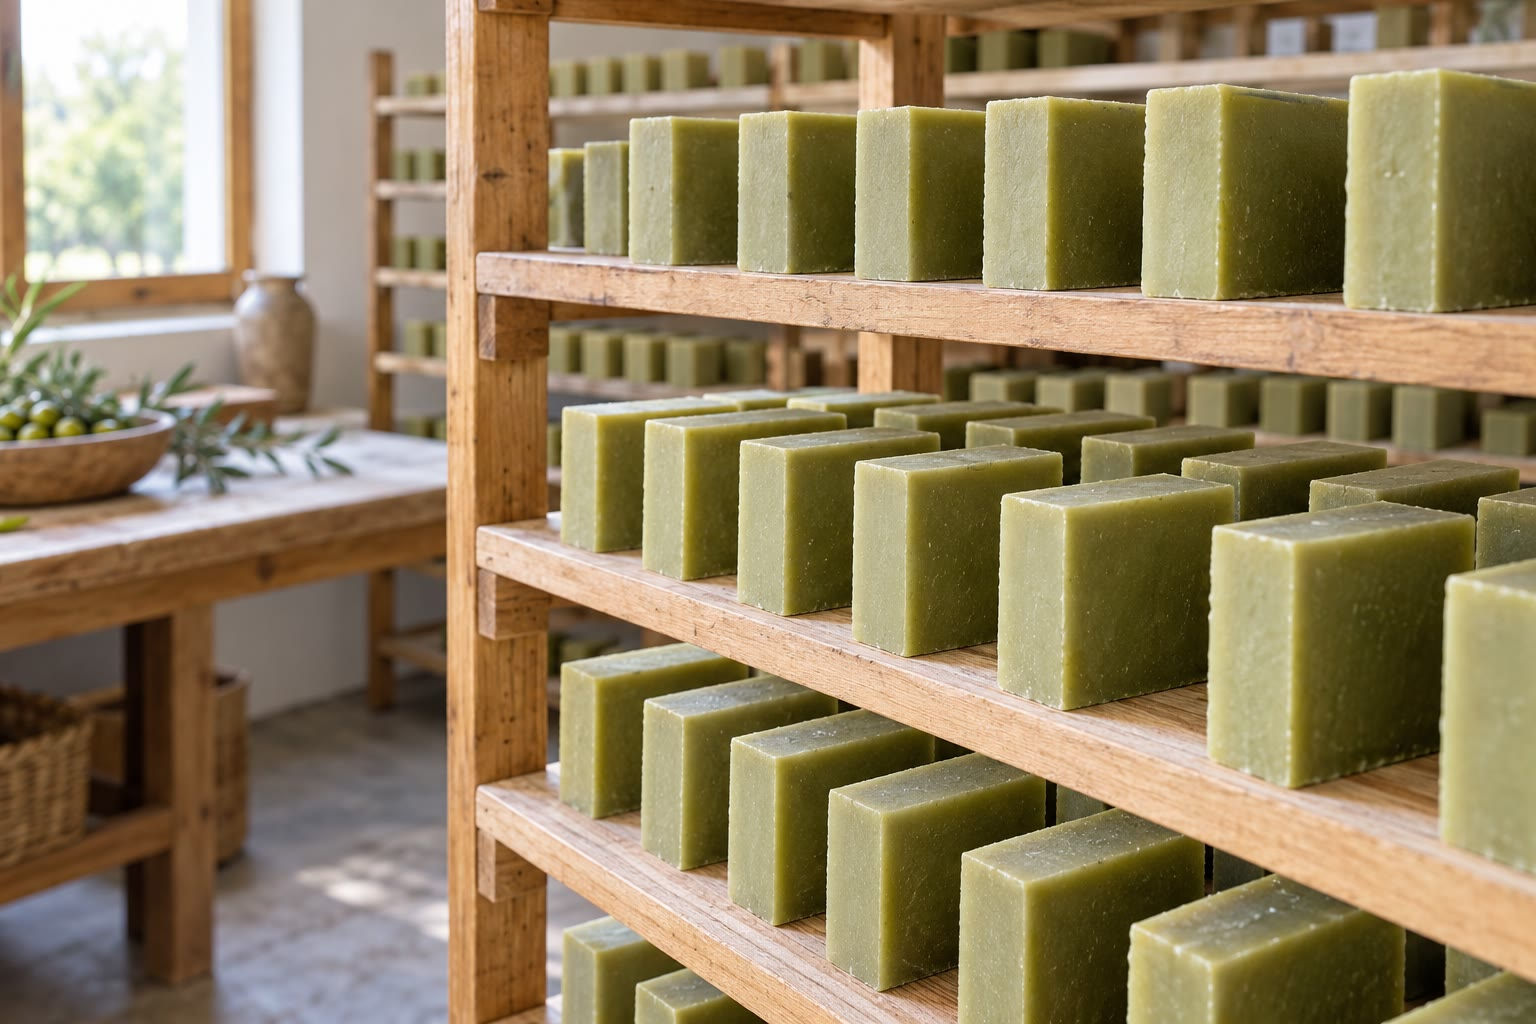
\includegraphics[width=0.58\linewidth]{images/book3/ai/b2-24-soap-bars.jpg}

{\small Pastillas de jabón de aceite de oliva secándose en estantes de madera. El jabón es la sal de sodio de los ácidos grasos
liberados cuando el aceite, un éster, se hierve con hidróxido de sodio.}
\end{omfigure}

\section{La familia y su reactividad}

\begin{definition}[Derivados de los ácidos carboxílicos]\label{def:b2:acyl-substitution:derivative}
Un \emph{derivado de ácido carboxílico}\index{derivado de acido carboxilico@derivado de ácido carboxílico} es un compuesto \ce{R-CO-Z} en
el que el \ce{OH} de un ácido carboxílico está sustituido por otro grupo Z. El \emph{grupo
acilo}\index{grupo acilo} $\mathrm{R{-}CO{-}}$ es común a todos ellos. En un \emph{cloruro de acilo}\index{cloruro de acilo},
Z es Cl; en un \emph{anhídrido de ácido}\index{anhidrido de acido@anhídrido de ácido}, Z es $\mathrm{O{-}CO{-}R'}$: dos grupos
acilo comparten un oxígeno; en un éster Z es $\mathrm{OR'}$, y en una amida, $\mathrm{NR'_2}$.
\end{definition}

\begin{proposition}[Escala de reactividad]\label{prop:b2:acyl-substitution:reactivity}
Frente a los nucleófilos, los derivados reaccionan en el orden \omterm{def:b2:acyl-substitution:derivative}{cloruro de acilo} $>$ anhídrido $>$ éster
$\approx$ ácido $>$ amida.
\end{proposition}

\begin{proof}[Argumento]
Se suman dos efectos. El grupo saliente \ce{Z-} sale tanto más fácilmente cuanto más débil es como base:
\ce{Cl-} (ácido conjugado \ce{HCl}, $\mathrm pK_a$ de unos $-7$) mucho mejor que un carboxilato
($\mathrm pK_a$ de unos 5), un alcóxido (unos 16) o un ion amiduro (unos 35). Y el grupo Z cede
densidad electrónica al carbonilo por donación mesómera de su par no enlazante, lo que hace al carbono
carbonílico menos electrófilo: débil para Cl, máxima para el nitrógeno. La amida es a la vez el electrófilo
más pobre y el peor grupo saliente.
% ledger: pka:ethanoic, pka:ethanol
\end{proof}

\section{Sustitución nucleófila de acilo}

\begin{definition}[Sustitución nucleófila de acilo]\label{def:b2:acyl-substitution:nas}
Una \emph{sustitución nucleófila de acilo}\index{sustitucion nucleofila de acilo@sustitución nucleófila de acilo} sustituye el grupo Z
de un compuesto acílico por un nucleófilo. Transcurre por adición del nucleófilo al carbono
carbonílico, que da un \emph{intermedio tetraédrico}\index{intermedio tetraedrico@intermedio tetraédrico}, seguida de la
eliminación del grupo saliente, que restaura el enlace \ce{C=O}.
\end{definition}

\begin{proposition}[Adición--eliminación]\label{prop:b2:acyl-substitution:addition-elimination}
La sustitución de acilo pasa por un \omterm{def:b2:acyl-substitution:nas}{intermedio tetraédrico}; se acelera en medio básico con un nucleófilo
más fuerte y en medio ácido por activación del carbonilo.
\end{proposition}

\begin{proof}[Argumento]
El carbono carbonílico, plano y electrófilo, acepta el nucleófilo por encima o por debajo de su
plano, como en las adiciones del \cref{ch:b2:amines}; con un grupo Z capaz de salir, el intermedio
lo expulsa en lugar de protonarse. En medio básico el nucleófilo es un anión (\ce{HO-},
\ce{RO-}); en medio ácido el oxígeno carbonílico se protona y basta un nucleófilo neutro (el agua, un
alcohol). Los ésteres marcados con \ce{^{18}O} en la parte alcohólica dan, por hidrólisis, alcohol marcado
y ácido sin marcar: el enlace que se rompe es el enlace acilo--oxígeno, como exige el mecanismo.
\end{proof}

\begin{omfigure}
\setchemfig{atom sep=1.7em}
\schemestart
\chemfig{R-C(=[2]O)-OR'} \+ \chemfig{HO^{-}}
\arrow{->[adición]}
\chemfig{R-C(-[2]O^{-})(-[6]OH)-OR'}
\arrow{->[eliminación]}[,1.3]
\chemfig{R-C(=[2]O)-OH} \+ \chemfig{^{-}OR'}
\schemestop

\medskip
\schemestart
\chemfig{R-C(=[2]O)-OH} \+ \chemfig{^{-}OR'}
\arrow{->[transferencia de protón]}
\chemfig{R-C(=[2]O)-O^{-}} \+ \chemfig{HOR'}
\schemestop
\par\vspace{6pt}

{\small \omterm{def:b2:acyl-substitution:saponification}{Saponificación} de un éster. El hidróxido se adiciona al carbono carbonílico, dando el \omterm{def:b2:acyl-substitution:nas}{intermedio
tetraédrico}; el alcóxido sale y el enlace \ce{C=O} se forma de nuevo; el alcóxido, una base fuerte, toma después
el protón del ácido. Esta última etapa hace que la reacción sea total.}
\end{omfigure}

\begin{method}[Escribir una sustitución de acilo]\label{met:b2:acyl-substitution:nas-mechanism}
\begin{enumerate}
  \item En medio básico: el nucleófilo aniónico se adiciona al carbono carbonílico; la carga negativa pasa al
        oxígeno; el enlace \ce{C=O} se forma de nuevo y Z sale; termínese con la etapa ácido--base que haya.
  \item En medio ácido: protónese el oxígeno carbonílico; el nucleófilo neutro se adiciona; transfiérase un protón
        al grupo saliente; este sale como molécula neutra; desprotónese el carbonilo.
  \item Cuéntense las etapas: cada intermedio es o bien tetraédrico o bien un compuesto carbonílico.
\end{enumerate}
\end{method}

\section{Ésteres}

\begin{definition}[Esterificación]\label{def:b2:acyl-substitution:esterification}
Una \emph{esterificación}\index{esterificacion@esterificación} forma un éster a partir de un ácido carboxílico (o de un derivado más
reactivo) y un alcohol. La reacción directa de un ácido con un alcohol, catalizada por un
ácido fuerte, es la esterificación de Fischer.
\end{definition}

\begin{proposition}[Esterificación de Fischer]\label{prop:b2:acyl-substitution:fischer}
La \omterm{def:b2:acyl-substitution:esterification}{esterificación} de Fischer es un equilibrio lento, con una constante cercana a 4 para los alcoholes primarios;
se desplaza en sentido directo con un exceso de uno de los reactivos o eliminando el agua a medida que se forma.
\end{proposition}

\begin{proof}[Argumento]
Etanol y ácido etanoico equimolares se detienen cuando se han esterificado dos tercios del ácido: $K =
(2/3)^2/(1/3)^2 = 4$. Si se mantiene $Q < K$ con un exceso de alcohol, o destilando el agua
(el aparato de Dean--Stark del volumen del primer año), la reacción avanza más
(\cref{ch:b2:equilibrium-shifts}). Las seis etapas del mecanismo son las del \cref{met:b2:acyl-substitution:nas-mechanism}
en medio ácido, todas reversibles.
% ledger: ester:berthelot
\end{proof}

\begin{definition}[Saponificación]\label{def:b2:acyl-substitution:saponification}
Una \emph{saponificación}\index{saponificacion@saponificación} es la hidrólisis de un éster por un hidróxido, que da
la sal carboxilato y el alcohol.
\end{definition}

\begin{proposition}[La saponificación es total]\label{prop:b2:acyl-substitution:saponification}
La \omterm{def:b2:acyl-substitution:saponification}{saponificación} es total: su última etapa, la transferencia de protón del ácido carboxílico al
alcóxido, tiene una constante de equilibrio del orden de $10^{11}$.
\end{proposition}

\begin{proof}
Para $\mathrm{RCOOH + R'O^- \to RCOO^- + R'OH}$,
\[
  K = \frac{K_a(\ce{RCOOH})}{K_a(\mathrm{R'OH})} = 10^{\mathrm pK_a(\mathrm{R'OH}) - \mathrm pK_a(\ce{RCOOH})} ;
\]
con el ácido etanoico (4.76) y el etanol (15.93), $K = 10^{11.2}$. El carboxilato, un electrófilo pobre, no es atacado por el alcohol: la reacción
global no retrocede.
% ledger: pka:ethanoic, pka:ethanol
\end{proof}

\begin{omfigure}
\setchemfig{atom sep=1.7em}
\schemestart
\chemfig{CH_2(-[0]O-CO-R)-[6]CH(-[0]O-CO-R)-[6]CH_2-[0]O-CO-R}
\+ \chemfig{3\,NaOH}
\arrow{->[calor]}
\chemfig{CH_2(-[0]OH)-[6]CH(-[0]OH)-[6]CH_2-[0]OH}
\+ \chemfig{3\,R-COO^{-}\,Na^{+}}
\schemestop
\par\vspace{6pt}

{\small \omterm{def:b2:acyl-substitution:saponification}{Saponificación} de un triglicérido: se cortan los tres enlaces éster, lo que da glicerol y
tres moléculas del carboxilato de sodio, el jabón (R es una cadena larga, \ce{C17H33} para el oleato del
aceite de oliva).}
\end{omfigure}

\begin{definition}[Transesterificación]\label{def:b2:acyl-substitution:transesterification}
Una \emph{transesterificación}\index{transesterificacion@transesterificación} intercambia la parte alcohólica de un éster,
$\mathrm{RCOOR' + R''OH \rightleftharpoons RCOOR'' + R'OH}$, con catálisis ácida o básica.
\end{definition}

\begin{definition}[Lactonas y lactamas]\label{def:b2:acyl-substitution:lactone}
Una \emph{lactona}\index{lactona} es un éster cíclico, formado por \omterm{def:b2:acyl-substitution:esterification}{esterificación} interna de un
hidroxiácido; una \emph{lactama}\index{lactama} es una amida cíclica.
\end{definition}

\section{Derivados activados}

Bajar por la escala de reactividad es fácil: un \omterm{def:b2:acyl-substitution:derivative}{cloruro de acilo} da un anhídrido, un éster o una
amida con el nucleófilo adecuado, a menudo a temperatura ambiente. Subir requiere una activación: un
ácido carboxílico se convierte en su cloruro con cloruro de tionilo,
\[
  \ce{RCOOH + SOCl2 -> RCOCl + SO2 + HCl} ,
\]
cuyos subproductos son gases. El \omterm{def:b2:acyl-substitution:derivative}{cloruro de acilo} reacciona después con un alcohol o con una amina; una base
(piridina, trietilamina o un segundo equivalente de la amina) atrapa el \ce{HCl} formado, que
de otro modo protonaría la amina.

\begin{method}[Moverse entre los derivados]\label{met:b2:acyl-substitution:ladder}
\begin{enumerate}
  \item Bajando por la escala (cloruro $\to$ anhídrido $\to$ éster, ácido $\to$ amida): trátese con el
        nucleófilo, con una base que capte el ácido liberado.
  \item Subiendo por la escala: conviértase primero el ácido en el cloruro (\ce{SOCl2}); un éster o una amida
        se hidroliza primero al ácido.
  \item Entre un ácido y un éster: \omterm{def:b2:acyl-substitution:esterification}{esterificación} de Fischer (equilibrio) o \omterm{def:b2:acyl-substitution:saponification}{saponificación}
        (total) seguida de acidificación.
\end{enumerate}
\end{method}

\begin{omfigure}
\begin{tikzpicture}[font=\small, >={Stealth}]
  \foreach \y/\n in {4/{cloruro de acilo \ce{RCOCl}}, 3/{anhídrido \ce{(RCO)2O}}, 2/{éster $\mathrm{RCOOR'}$ \quad ácido \ce{RCOOH}}, 1/{amida $\mathrm{RCONR'_2}$}} {
    \node[cyclenode, minimum width=5.2cm] at (0,\y*1.1) {\n};
  }
  \draw[->, thick, omDef] (-3.1,4.3) -- (-3.1,1.1) node[midway, left, align=right, font=\scriptsize] {fácil:\\ nucleófilo\\ + base};
  \draw[->, thick, omThm] (3.1,2.2) -- (3.1,4.4) node[midway, right, align=left, font=\scriptsize] {cuesta arriba:\\ vía el ácido\\ y \ce{SOCl2}};
  \node[font=\scriptsize, anchor=south] at (0,4.85) {más reactivo};
  \node[font=\scriptsize, anchor=north] at (0,0.55) {menos reactivo};
\end{tikzpicture}

{\small La escala de reactividad de los derivados de los ácidos carboxílicos. Cualquier derivado puede convertirse en
uno situado más abajo mediante un nucleófilo; para subir se pasa por el ácido y su cloruro.}
\end{omfigure}

\section{Organometálicos e hidruros}

\begin{proposition}[Dos adiciones de Grignard]\label{prop:b2:acyl-substitution:grignard-ester}
Un éster tratado con un exceso de organomagnesiano da un alcohol terciario que lleva dos
grupos idénticos procedentes del reactivo.
\end{proposition}

\begin{proof}[Argumento]
La primera adición da un \omterm{def:b2:acyl-substitution:nas}{intermedio tetraédrico} que expulsa el alcóxido: una cetona. Una cetona
es más electrófila que un éster (no hay donación mesómera de un grupo $\mathrm{OR'}$) y reacciona con
el reactivo más deprisa que el éster restante; la segunda adición, a la cetona, da el alcóxido
de un alcohol terciario, que el tratamiento ácido protona. La reacción no puede detenerse en la cetona.
\end{proof}

\begin{proposition}[Reducciones con hidruros]\label{prop:b2:acyl-substitution:hydrides}
El hidruro de litio y aluminio reduce los ésteres y los ácidos a alcoholes primarios, y las amidas a aminas;
el borohidruro de sodio reduce los aldehídos y las cetonas, pero no los ésteres, los ácidos ni las amidas. Un hidruro de aluminio
voluminoso (DIBAL-H) a \qty{-78}{\degreeCelsius} reduce un éster al aldehído.
\end{proposition}

\begin{proof}[Argumento]
\ce{LiAlH4} es un dador de hidruro fuerte: como el reactivo de Grignard, se adiciona dos veces a un éster (pasando por
el aldehído). El borohidruro es demasiado débil para el carbonilo del éster, menos electrófilo. Con DIBAL-H a
baja temperatura, el \omterm{def:b2:acyl-substitution:nas}{intermedio tetraédrico}, retenido por el aluminio, no expulsa el alcóxido hasta
el tratamiento acuoso, cuando ya no queda hidruro: el aldehído sobrevive. En una amida, el oxígeno,
unido al aluminio, se elimina en lugar del nitrógeno, y deja un ion iminio que el hidruro
reduce a la amina.
\end{proof}

\begin{history}[Chevreul y las grasas]
\begin{minipage}[t]{0.22\linewidth}
\vspace{0pt}
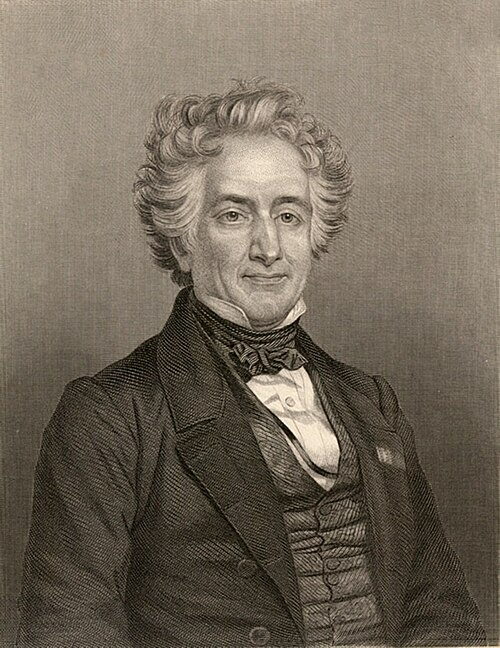
\includegraphics[width=\linewidth]{images/book3/chevreul.jpg}
\end{minipage}\hfill
\begin{minipage}[t]{0.74\linewidth}
\vspace{0pt}
Michel Eugène Chevreul demostró, en un estudio publicado en 1823, que las grasas son compuestos del glicerol
con ácidos grasos, que él aisló y nombró (ácidos esteárico, oleico, butírico), y que la
\omterm{def:b2:acyl-substitution:saponification}{saponificación} las divide en esas dos partes. Su trabajo convirtió la fabricación de jabones y velas en
química; vivió hasta los 102 años. (Retrato de Nicolas Eustache Maurin, dominio público, Wikimedia
Commons.)
\end{minipage}
\end{history}

\begin{safety}{\ghs[5mm]{GHS02}\,\ghs[5mm]{GHS05}\,\ghs[5mm]{GHS06}}
El cloruro de tionilo y los \omterm{def:b2:acyl-substitution:derivative}{cloruros de acilo} reaccionan violentamente con el agua y desprenden gases corrosivos;
se manipulan en seco, en una vitrina de gases. El hidruro de litio y aluminio se inflama en contacto con el agua; su
exceso se destruye con cuidado al final. El hidróxido de sodio concentrado es corrosivo para la piel y los
ojos. El metanol es tóxico e inflamable.
% ledger: ghs:SOCl2, ghs:ethanoyl-chloride, ghs:LiAlH4, ghs:NaOH, ghs:methanol
\end{safety}

\section{Ejercicios}

\begin{exercise}[$\star$]\label{exo:b2:acyl-substitution:1}
Ordénense por reactividad frente al agua: etanoato de etilo, cloruro de etanoílo, etanamida, anhídrido
etanoico.
\end{exercise}

\begin{exercise}[$\star$]\label{exo:b2:acyl-substitution:2}
Dense los productos del cloruro de etanoílo con: agua; etanol; amoníaco (2 equivalentes);
etanoato de sodio; dimetilamina con trietilamina.
\end{exercise}

\begin{exercise}[$\star$]\label{exo:b2:acyl-substitution:3}
Escríbase la \omterm{def:b2:acyl-substitution:saponification}{saponificación} del benzoato de metilo por el hidróxido de sodio y calcúlese la masa de hidróxido
de sodio necesaria para \qty{13.6}{g} del éster.
\end{exercise}

\begin{exercise}[$\star$]\label{exo:b2:acyl-substitution:4}
Dibújese la \omterm{def:b2:acyl-substitution:lactone}{lactona} formada por el ácido 4-hidroxibutanoico e indíquese el tamaño de su anillo.
\end{exercise}

\begin{exercise}[$\star\star$]\label{exo:b2:acyl-substitution:5}
Escríbase el mecanismo de la reacción del etanoato de etilo con el amoníaco.
\end{exercise}

\begin{exercise}[$\star\star$]\label{exo:b2:acyl-substitution:6}
La aspirina se prepara a partir del ácido salicílico (ácido 2-hidroxibenzoico) y el anhídrido etanoico. ¿Qué grupo
del ácido salicílico reacciona, y cuál es el subproducto?
\end{exercise}

\begin{exercise}[$\star\star$]\label{exo:b2:acyl-substitution:7}
El etanoato de etilo se trata con un exceso de bromuro de metilmagnesio y luego con ácido diluido. Dese el
producto y explíquese por qué no puede aislarse la cetona.
\end{exercise}

\begin{exercise}[$\star\star$]\label{exo:b2:acyl-substitution:8}
Dese el producto de la reducción de la \omterm{def:b2:acyl-substitution:lactone}{lactona} del ejercicio 4 por \ce{LiAlH4}.
\end{exercise}

\begin{exercise}[$\star\star$]\label{exo:b2:acyl-substitution:9}
Con $K = 4$, calcúlese la fracción de ácido etanoico esterificada con uno y luego con tres
equivalentes de etanol. ¿Qué otro método desplaza la reacción?
\end{exercise}

\begin{exercise}[$\star\star\star$]\label{exo:b2:acyl-substitution:10}
Prepárese la \textit{N},\textit{N}-dietilbenzamida a partir del ácido benzoico, y explíquese por qué mezclar el ácido
con dietilamina y calentar suavemente da en cambio una sal.
\end{exercise}

\begin{exercise}[$\star\star\star$]\label{exo:b2:acyl-substitution:11}
El índice de \omterm{def:b2:acyl-substitution:saponification}{saponificación} de una grasa es la masa de hidróxido de potasio, en mg, necesaria para saponificar
\qty{1}{g} de ella. Calcúlese para la trioleína (\qty{885.4}{g/mol}; KOH \qty{56.11}{g/mol}).
\end{exercise}

\begin{exercise}[$\star\star\star$]\label{exo:b2:acyl-substitution:12}
Una molécula lleva un éster, una amida y una cetona. ¿Qué grupo(s) reduce el \ce{NaBH4}, y cuáles
el \ce{LiAlH4}? ¿Qué se obtiene en cada caso?
\end{exercise}

\section{Problema: biodiésel a partir de aceite de fritura}

\begin{problem}[{Problema de fin de semana --- la trioleína y su masa molar, su transesterificación con
metanol y el papel de la base, la reacción secundaria con los ácidos libres y el agua, y los rendimientos por
tonelada de aceite}]
\label{pb:b2:acyl-substitution:1}
Modélese el aceite como trioleína pura, el triglicérido del ácido oleico (\ce{C17H33COOH}). Masas molares
(\unit{g/mol}): C 12.011, H 1.008, O 15.999, Na 22.990. El glicerol es el propano-1,2,3-triol.
% ledger: aw:C, aw:H, aw:O, aw:Na, ghs:methanol, ghs:NaOH

\medskip
\noindent\textbf{Parte I --- La trioleína.}
\begin{enumerate}
  \item Dense las fórmulas del ácido oleico y del glicerol.
  \item Escríbase la fórmula de la trioleína y calcúlese su masa molar.
  \item ¿Cuántos grupos éster contiene?
  \item El ácido oleico tiene un doble enlace cis. ¿Por qué los aceites ricos en él son líquidos a temperatura ambiente?
  \item ¿Qué daría la \omterm{def:b2:acyl-substitution:saponification}{saponificación} de la trioleína?
  \item ¿Qué es químicamente el biodiésel?
\end{enumerate}

\medskip
\noindent\textbf{Parte II --- \omterm{def:b2:acyl-substitution:transesterification}{Transesterificación}.}
\begin{enumerate}[resume]
  \item Escríbase la \omterm{def:b2:acyl-substitution:transesterification}{transesterificación} de la trioleína con metanol.
  \item ¿Por qué se usa una base (metóxido o hidróxido de sodio) como catalizador?
  \item Dibújese el \omterm{def:b2:acyl-substitution:nas}{intermedio tetraédrico} del primer intercambio.
  \item ¿Por qué se usa metanol en exceso (seis equivalentes en lugar de tres)?
  \item El glicerol no es miscible con los ésteres metílicos. ¿En qué ayuda esto?
  \item ¿Se consume el catalizador en la reacción ideal?
\end{enumerate}

\medskip
\noindent\textbf{Parte III --- Ácidos libres y agua.}
\begin{enumerate}[resume]
  \item El aceite de fritura usado contiene ácido oleico libre. ¿Qué le hace a la base?
  \item ¿Qué les hace el agua a los ésteres metílicos en presencia de la base?
  \item ¿Por qué es un estorbo el jabón formado?
  \item ¿Cómo pueden eliminarse primero los ácidos libres, sin base?
  \item ¿Por qué debe secarse el aceite antes de la reacción?
\end{enumerate}

\medskip
\noindent\textbf{Parte IV --- Por tonelada de aceite.}
\begin{enumerate}[resume]
  \item Calcúlese la cantidad de trioleína en una tonelada.
  \item Calcúlese la masa de metanol consumida.
  \item Calcúlese la masa de oleato de metilo formada.
  \item Compruébese la conservación de la masa.
  \item Un aceite con un 2~\% en masa de ácido oleico libre se trata con hidróxido de sodio: calcúlese la masa de
        hidróxido de sodio que consume el ácido por tonelada.
  \item Calcúlese la masa de glicerol coproducida por tonelada de trioleína.
\end{enumerate}
\end{problem}
